\documentclass[12pt]{beamer}
\usepackage[english, russian]{babel}
\usepackage[utf8x]{inputenc}
\usepackage{itmobeamer}
\usepackage{makecell}

\title[Исследование и реаализация ДО CBWFQ]{Исследование и реализация взвешенного алгоритма честного обслуживания на основе классов}
\author[]{Куклина Мария}
\institute[]{Университет ИТМО}
\date[]{Санкт-Петербург, 2018}

\begin{document}

%\itmologoslide

\begin{darkbars}
    \begin{frame}[noheader,nologo,noframenumbering]
        \titlepage
    \end{frame}
\end{darkbars}

%\begin{frame}[rulogoheader,nologo,noframenumbering]
%    \itmoanothertitle
%\end{frame}

\begin{frame}{Цели и задачи}
    Цель -- реализация дисциплины обслуживания Class-Based Weighted Fair Queueing
    (CBWFQ) в ядре Linux.
    
    Задачи.
    {\small
        \begin{itemize}
            \item Провести сравнительный анализ CBWFQ с рядом выбранных дисциплин обслуживания.
            \item Настроить среду для реализации и тестирования.
            \item Реализовать CBWFQ в ядре Linux.
            \item Добавить интерфейс в утилиту tc для работы с ДО.
        \end{itemize}
    }
\end{frame}

\begin{frame}{Quality of Serivce}
\end{frame}

\begin{frame}{Priority Queueing}
	%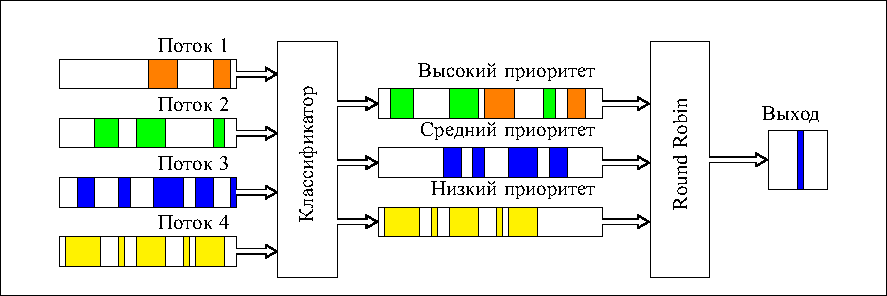
\includegraphics{../../text/src/pdfimages/pq.pdf}
\end{frame}

\begin{frame}{Class Based Queueing}
\end{frame}

\begin{frame}{Hierarchy Token Bucket}
\end{frame}

\begin{frame}{HFSC}
\end{frame}
\begin{frame}{Flow-based Weighted Fair Queueing}
\end{frame}
\begin{frame}{Class-Based Weighted Fair Queueing}
\end{frame}

\newcommand{\mc}[0]{\makecell}
\begin{frame}{Сравнительная таблица ДО}
{\footnotesize
    \begin{tabular}{|c|c|c|c|c|c|c|}
        \hline
               Свойство     & PQ   & CBQ   & HTB   & HFSC  & FWFQ  & CBWFQ \\ \hline
\mc{Метод\\ планирования}   & RR   & RR    & RR    & RT/LS & WFQ   & WFQ   \\ \hline
Честность                   & -    & -     & -     & +     &  +    &  +    \\ \hline
     Отбрасывание           & TD   & TD    & TD    & TD    & ED/AD & TD/WRED \\ \hline
\mc{Разделение\\ канала}    & -    &  +    &  +    &  +    &  -    &  -    \\ \hline
\mc{Сложность \\ реализации}& L    & H     &  M    &  H    &   M   &  M\\ \hline
    \end{tabular}
}

{\scriptsize
	Обозначения:\\
	 H -- высокий, M -- средний, L -- низкий; \\
	 RR -- Round Robin, RT/LS -- на основе Real Time/Link Sharing критериев.\\
	 TD -- Tail Drop, ED -- Early Dropping, ED -- Aggressive Dropping.
}
\end{frame}

\begin{frame}{Подсистема Traffic Control в ядре Linux}
\end{frame}

\begin{frame}{Схемы в AnyLogic}
\end{frame}

\begin{frame}{Вывод}
\end{frame}

%\begin{frame}[nologo]
%\end{frame}

\itmothankyou

\end{document}

